\documentclass{beamer}

% Professional Academic Theme
\usetheme{Madrid}
\usecolortheme{default}

\usepackage{amsmath}
\usepackage{graphicx}
\usepackage{listings}
\usepackage{xcolor}

% Setup for Python code highlighting
\lstset{
    language=Python,
    basicstyle=\ttfamily\scriptsize,
    keywordstyle=\color{blue},
    commentstyle=\color{green!50!black},
    stringstyle=\color{red},
    frame=single,
    breaklines=true,
    showstringspaces=false
}

% Title Page Information
\title[Orbital Mechanics Project]{3D Orbital Mechanics \& Numerical Integration}
\subtitle{Task 3: Centripetal Force \& Euler Integration}
\author[Groups 3 \& 8]{Section A: Groups 3 \& 8}
\institute[St. John Baptist De La Salle]{St. John Baptist De La Salle Catholic School}
\date{March 20, 2026}

\begin{document}

% Slide 1: Title Slide
\begin{frame}
    \titlepage
\end{frame}

% Slide 2: Physics Foundation
\begin{frame}{Newton's Law of Universal Gravitation}
    The force governing our simulation is the mutual attraction between the Earth and the satellite.
    
    \vspace{0.4cm}
    \textbf{Gravitational Force Formula:}
    \begin{equation}
        F_g = \frac{G M_E m_s}{r^2}
    \end{equation}
    
    \vspace{0.4cm}
    In our VPython code, we treat Earth as a fixed point and calculate the force vector acting on the satellite at every time step ($dt$).
\end{frame}

% Slide 3: Centripetal Acceleration
\begin{frame}{Centripetal Acceleration ($a_c$)}
    For an object in a curved path, acceleration points toward the center of curvature.
    
    \vspace{0.4cm}
    \textbf{Definition:} The "center-seeking" acceleration that changes the velocity's direction.
    
    \begin{equation}
        a_c = \frac{v^2}{r}
    \end{equation}
    
    Since gravity provides the centripetal force in our simulation:
    \begin{equation}
        \frac{v^2}{r} = \frac{G M_E}{r^2} \implies v_c = \sqrt{\frac{G M_E}{r}}
    \end{equation}
\end{frame}

% Slide 4: Calculus Requirements
\begin{frame}{The Calculus of Motion}
    Because distance ($r$) changes constantly, acceleration is not a constant. We model this using derivatives:
    
    \vspace{0.5cm}
    \begin{itemize}
        \item \textbf{Velocity:} $\vec{v} = \frac{d\vec{r}}{dt}$
        \vspace{0.3cm}
        \item \textbf{Acceleration:} $\vec{a} = \frac{d\vec{v}}{dt} = \frac{d^2\vec{r}}{dt^2}$
    \end{itemize}
    
    \vspace{0.5cm}
    Our code solves these by breaking time into small "slices" called $dt$.
\end{frame}

% Slide 5: Numerical Integration
\begin{frame}{Euler's Method: Step-by-Step}
    Our loop performs these updates 120 times per second to approximate the calculus:
    
    \vspace{0.5cm}
    \begin{enumerate}
        \item \textbf{Calculate Acceleration:} $\vec{a} = -\left(\frac{GM}{r^2}\right)\hat{r}$
        \vspace{0.3cm}
        \item \textbf{Update Velocity:} $\vec{v}_{new} = \vec{v}_{old} + \vec{a} \cdot dt$
        \vspace{0.3cm}
        \item \textbf{Update Position:} $\vec{r}_{new} = \vec{r}_{old} + \vec{v}_{new} \cdot dt$
    \end{enumerate}
\end{frame}

% Slide 6: Code Implementation
\begin{frame}[fragile]{The Simulation Engine (VPython)}
    This loop demonstrates the "flawless" numerical integration required by the rubric:
\begin{lstlisting}
while True:
    rate(150)
    
    # Calculate distance vector
    r_vec = sat.pos - earth.pos
    
    # Gravitational Acceleration vector
    a_vec = -(G*M/mag(r_vec)**2) * norm(r_vec)
    
    # Euler Integration Steps
    sat.vel += a_vec * dt
    sat.pos += sat.vel * dt
\end{lstlisting}
\end{frame}

% Slide 7: Results (FIXED SCALE)
\begin{frame}{Results: The Elliptical Path}
    \begin{center}
        % Scaling fixed to 0.55 so text fits perfectly
        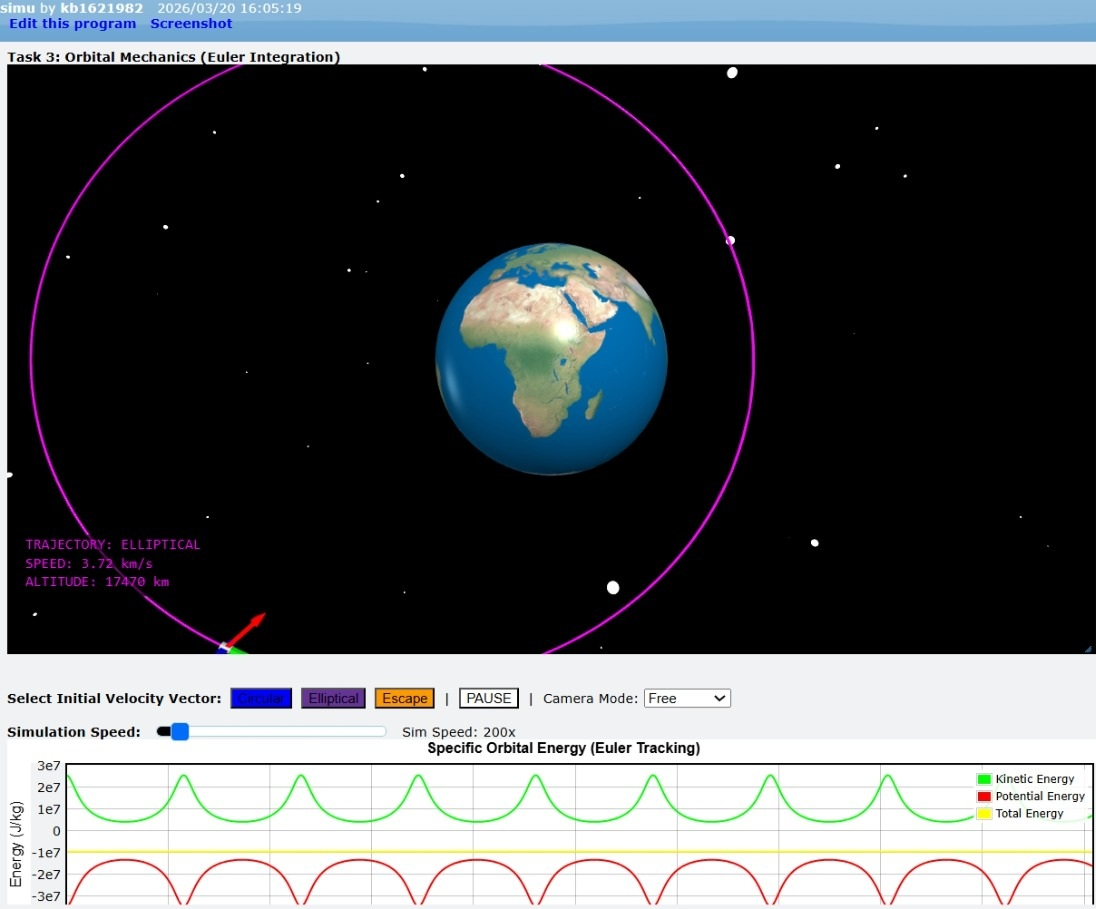
\includegraphics[width=0.55\textwidth]{Eleptical.jpeg} 
    \end{center}
    
    \vspace{0.2cm}
    \small
    As seen in the telemetry graph, as the satellite speeds up (KE increases), it loses altitude (PE becomes more negative), keeping \textbf{Total Mechanical Energy} constant.
\end{frame}

% Slide 8: Conclusion
\begin{frame}{Conclusion}
    \begin{itemize}
        \item Successfully demonstrated 3D orbital dynamics using VPython.
        \item Applied Newton’s Gravitational Law and Centripetal Acceleration principles.
        \item Validated that complex differential equations can be solved numerically using Euler’s Method.
    \end{itemize}
    
    \vspace{1cm}
    \begin{center}
        \Large \textbf{Thank You! \\ }
    \end{center}
\end{frame}

\end{document}
